\section{Getting Started} \label{getting_started}
In \Voreen the user is working with so-called \emph{workspaces}. A workspace is a file ending with `\verb|*.vws|' which specifies a user-defined project. 
The file stores all important settings, e.g. which data sets have been loaded, the color map specification, or the camera orientation settings.\\
An example workflow of \Voreen could look like this:
\begin{itemize}
\item Open a \workspace (e.g. \verb|ultramicroscopy.vws|).
\item Work with the workspace, e.g.:
\begin{itemize}
	\item load data sets
	\item change color maps
	\item create an animation
\end{itemize}
\item Save the workspace under a user-defined name (e.g. \verb|myfirst_ultramicroscopy.vws|).
\end{itemize}
Once a workspace is saved it can be loaded to restore all of its settings. The \workspaces cannot be overwritten.

Throughout this section, the basic tools used in all of the \workspaces will be explained. 
For a more detailed description of the features related to a specific \workspace please refer to the associated sections of this document.

\subsection{Supported Data Formats}
\label{section:data_formats}

The current version of \Voreen supports data sets in the following formats:
\begin{itemize}
	\item \verb|*.tif| (Tagged Image File)
	\item \verb|*.ome.tif| (OME-TIFF)
	\item \verb|*.vvd| (Voreen Volume Data) 
\end{itemize}
\textbf{Note:} Currently \Voreen does not support time series / time-variant data. 

\subsection{The Interface}
\label{section:interface}

When starting up \Voreen for the first time, a startup workspace is loaded which provides some explanations to the general user interface 
of \Voreen and will be considered in detail throughout section \ref{section:startup_workspace}. The application should look similar to 
figure \ref{fig:vb_complete_interface}.

\begin{figure}[htb]
 \centering
 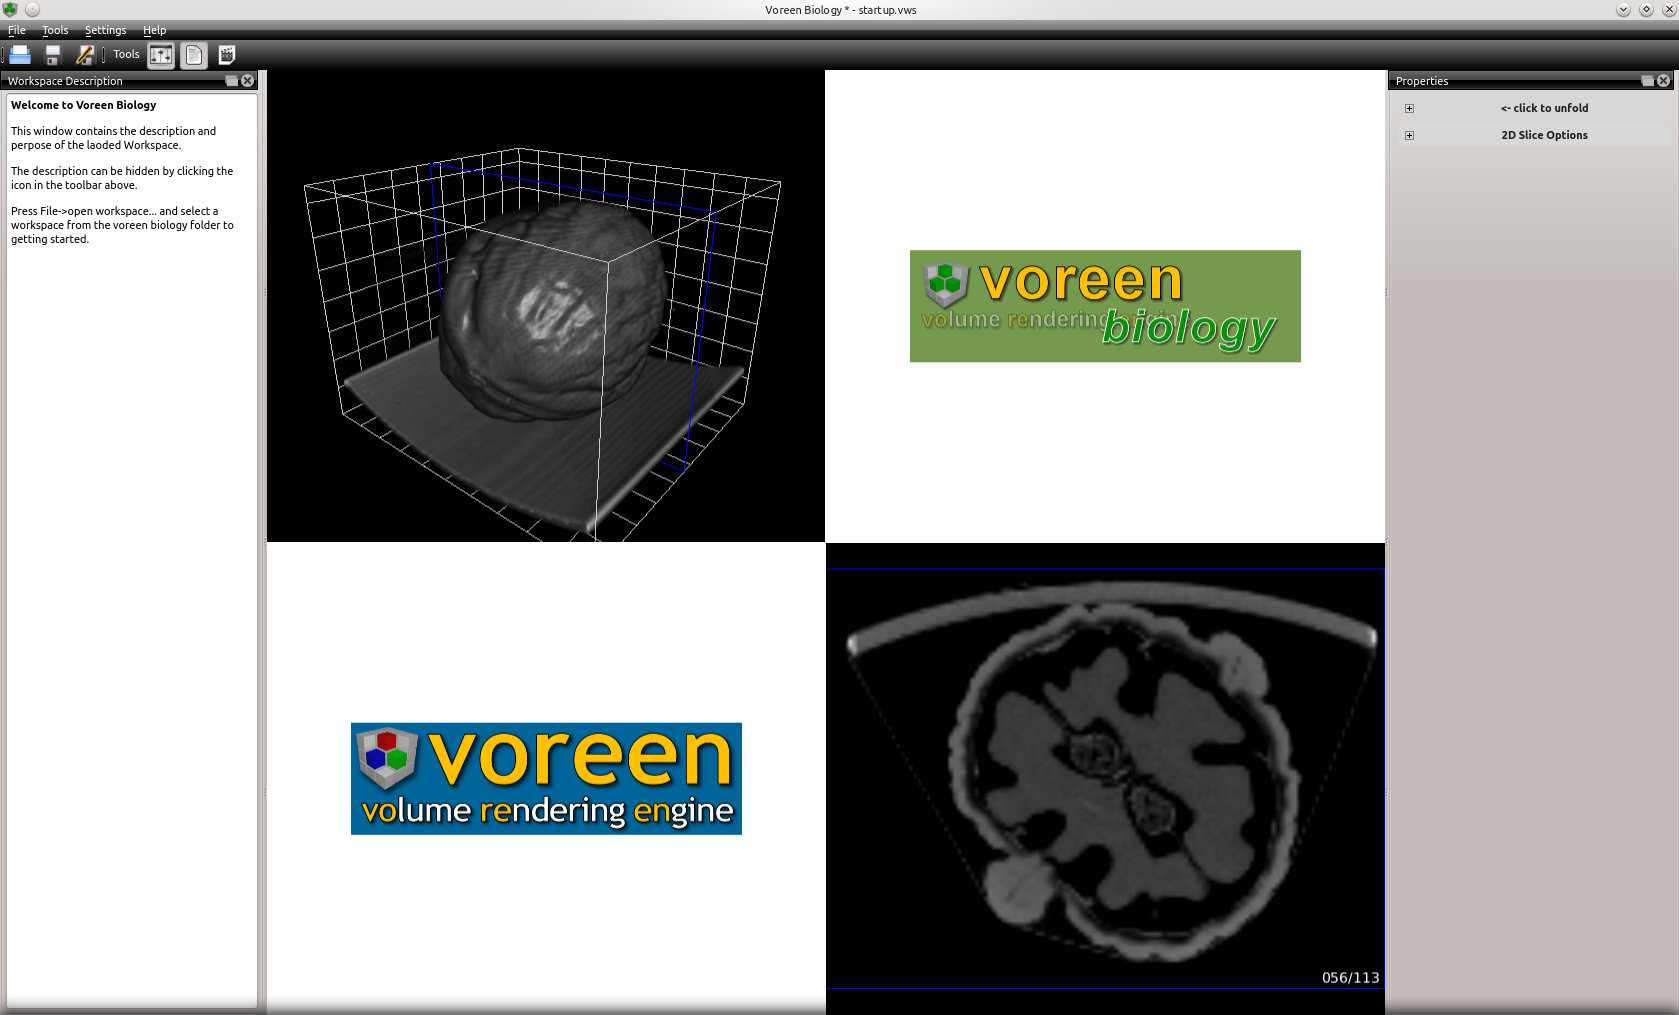
\includegraphics[scale=0.337,keepaspectratio=true]{./images/voreen_biology_complete_interface.png}
 % voreen_biology_complete_interface.png: 1679x1015 pixel, 90dpi, 47.39x28.65 cm, bb=0 0 1343 812
 \caption{\Voreen at the first start}
 \label{fig:vb_complete_interface}
\end{figure}

The interface of \Voreen consists of several parts. The central part is the \emph{quad view}, which contains four rendered images and allows the user 
to directly interact with the visualization. In many cases, it
will contain a three-dimensional rendering of the data set as well as three slice view renderings (one for each of the $xy$-, $yz$-, and $xz$-planes),
but it may also contain other visualizations, depending on the workspace. The quad view will be considered in detail during section \ref{section:quadview}.

The menu bar at the top of the \Voreen window, which is depicted in figure \ref{fig:menu_bar}, allows to open and save workspaces, 
as will be seen during the subsequent sections, and to change 
the global settings of the application, which are not workspace-dependent.

\begin{figure}[htb]
 \centering
 
\includegraphics[scale=1.1,keepaspectratio=true]{./images/menu_bar.png}
 % menu_bar.png: 174x18 pixel, 90dpi, 4.91x0.51 cm, bb=0 0 139 14
 \caption{The \Voreen menu bar}
 \label{fig:menu_bar}
\end{figure}

Below the menu bar, a tool bar, which is depicted in figure \ref{fig:tool_bar}, 
provides shortcut icons to the loading and saving functionality.
Additionally, it allows to enable or disable the display of the \emph{property window}, the \emph{workspace description window} and the \emph{animation window}.

\begin{figure}[htb]
 \centering
 
\includegraphics[scale=1.1,keepaspectratio=true]{./images/tool_bar.png}
 % tool_bar.png: 244x33 pixel, 90dpi, 6.89x0.93 cm, bb=0 0 195 26
 \caption{The \Voreen tool bar}
 \label{fig:tool_bar}
\end{figure}

The property window is located on the right side of the application and provides the functionality the change the settings of the workspace, i.e. the visualization
properties, such as the color map. The visualization properties are arranged in groups, which can be unfolded by clicking on the `+'-symbol as shown in figure 
\ref{fig:property_groups} to reveal the elements of the group.

\begin{figure}[htb]
 \centering
 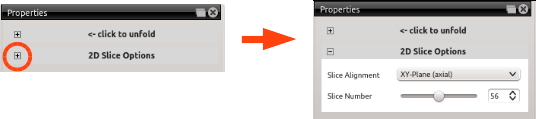
\includegraphics[scale=1.1,keepaspectratio=true]{./images/property_groups.png}
 % property_groups.png: 536x119 pixel, 96dpi, 14.18x3.15 cm, bb=0 0 402 89
 \caption{The property groups can be unfolded and folded to show and hide the visualization settings.}
 \label{fig:property_groups}
\end{figure}

The workspace description window provides information about the current workspace. It can be edited by the user to provide descriptions of the 
specific workspace settings, notes, etc. by using the right mouse button on the description window. 
The workspace description supports the use of \verb|html|-tags for formatting the description.

The rightmost icon in the tool bar opens and closes the \emph{animation editor}, which allows to animate the property settings of the workspace 
within a time frame, for instance allowing the user to create camera animations and to export this animation as a video or an image sequence.
The animation editor will be examined throughout section \ref{section:animation_editor}.

\subsection{Loading Workspaces}

To load a workspace in \Voreen, click on the `File'-menu at the upper left of the application, which is shown in figure \ref{fig:loading_workspaces}, 
then select the item `Open Workspace...'. A file dialog 
window will pop up where you can select a `\verb|*.vws|'-file to load. Additionally, opening the `File'-menu will display several recently loaded workspaces
at the bottom, which can be opened directly. 

\begin{figure}[htb]
 \centering
 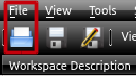
\includegraphics[scale=1.0,keepaspectratio=true]{./images/loading_workspaces_2.png}
 % loading_workspaces_1.png: 128x70 pixel, 90dpi, 3.61x1.98 cm, bb=0 0 102 56
 \caption{Loading workspaces}
 \label{fig:loading_workspaces}
\end{figure}
Alternatively, an icon for loading a workspace by opening the file dialog window is provided in the tool bar directly below 
the `File'-menu, as shown in figure \ref{fig:loading_workspaces}. 

If the current workspace has been modified by the user, a message box will show up which allows to save the changes made to the current workspace
before loading the selected file. This dialog is depicted in figure \ref{fig:loading_workspaces_message}.

\begin{figure}[htb]
 \centering
 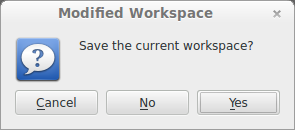
\includegraphics[scale=0.7,keepaspectratio=true]{./images/loading_workspaces_message.png}
 % loading_workspaces_message.png: 249x142 pixel, 90dpi, 7.03x4.01 cm, bb=0 0 199 114
 \caption{If changes have been made to the current workspace, \Voreen will display this message, allowing the user to save changes to the current workspace before loading the selected file, or to cancel the loading process.}
 \label{fig:loading_workspaces_message}
\end{figure}

\subsection{Saving Workspaces}

In \Voreen, workspaces can be saved in two ways. The user may either decide to save the changes made in the current workspace under the same name, i.e. set 
the new state to the current workspace file, or to save the modified workspace under a new name.
To save the changes in the current workspace file, click on the `File'-menu at the upper left of the application  
and select the item `Save Workspace'. 
To save the modified workspace under a new filename, instead of selecting `Save Workspace', select `Save Workspace As...' in the `File'-menu. 
This will open a file dialog where a directory and filename may be selected for the workspace. The file dialog also allows to select an already existing workspace file
for overwriting it with the current workspace.

Both saving features are also available to the user as icons in the tool bar, which are marked by the red box in figure \ref{fig:saving_workspaces}. 
The left icon refers to the `Save Workspace'-function while the right icon will open the `Save Workspace As...'-file dialog.

\begin{figure}[htb]
 \centering
 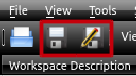
\includegraphics[scale=1.0,keepaspectratio=true]{./images/saving_workspaces_1.png}
 % loading_workspaces_1.png: 128x70 pixel, 90dpi, 3.61x1.98 cm, bb=0 0 102 56
 \caption{Saving workspaces}
 \label{fig:saving_workspaces}
\end{figure}
Please note that the \workspaces cannot be overwritten. Trying to save changes to such a workspace will always open a file dialog window. 

\subsection{The Quad View}
\label{section:quadview}

The quad view is the central component of the \Voreen visualization, as it provides the actual images of the data set and allows the user 
to explore the data via direct interaction with the canvas. 

By double-clicking with the left mouse button on one of the four components of the quad view the component is enlarged to fill the entire are of the quad
view, which is depicted in figure \ref{fig:quadview_resizing}. Using the double-click again will return to the regular quad view.

\begin{figure}[htb]
 \centering
 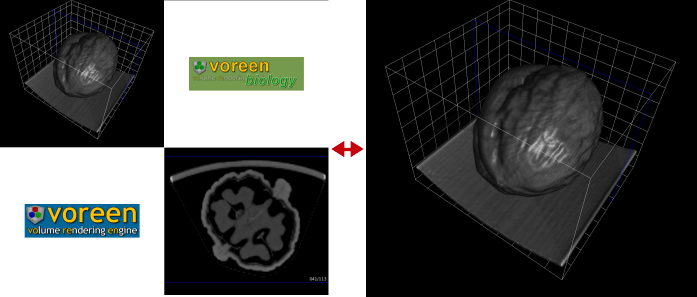
\includegraphics[scale=0.85,keepaspectratio=true]{./images/quadview_resizing2.png}
 % quadview_resizing.png: 697x297 pixel, 96dpi, 18.44x7.86 cm, bb=0 0 523 223
 \caption{Double-clicking with the left mouse button enlarges a single rendering canvas or returns to the regular quad view.}
 \label{fig:quadview_resizing}
\end{figure}

The quad view allows direct user interaction via use of the mouse buttons and movement and a few additional keys. The three-dimensional
rendering allows to rotate the camera using the \emph{trackball metaphor} by pressing the left mouse button and simply moving the mouse. By holding 
down the \verb|Ctrl|/\verb|Strg|-key, a continuous rotation is possible, which can be stopped by clicking the left mouse button. By holding down the 
\verb|Shift|-key, the camera position can be moved using the mouse instead of rotating the camera. The mouse wheel, or, alternatively, holding down 
the right mouse button while moving the mouse, allows zooming in and out. 

In the slice view, the mouse wheel, or, alternatively, holding down the mouse wheel and moving the mouse, will change the slice number, i.e. the location
along the image stack. By holding down the \verb|Ctrl|/\verb|Strg|-key, the center of the slice view regarding the slice can be shifted.

\subsection{Color Maps and Editor}
\label{section:color_map}

One of the most important properties in \Voreen is the color map, or \emph{transfer function}, editor. It is generally located in the property list window 
on the right side of the \Voreen application, which has already been mentioned in section \ref{section:interface}. Depending on the specific workspace,
several color map properties may exist, e.g. for specifying the color map of each of the individual channels of the data set individually, or for having separate
color map settings for the three-dimensional view and two-dimensional view. The basic color map property is depicted in figure \ref{fig:color_map_editor}.

\begin{figure}[htb]
 \centering
 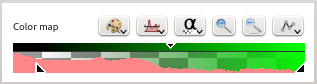
\includegraphics[scale=1.0,keepaspectratio=true]{./images/color_map_editor.png}
 % color_map_editor.png: 318x85 pixel, 90dpi, 8.98x2.40 cm, bb=0 0 254 68
 \caption{The color map property}
 \label{fig:color_map_editor}
\end{figure}

The property displays the intensity histogram of the data set as well as the color map mapped to the corresponding data values. With the use of the two sliders
at the bottom the domain of the color map can be changed. The slider on the top of the color map property can be used to adjust the gamma value. The icons on
the top of the color map property allow further adjustments of the color map. The leftmost icon opens a menu where several pre-defined color maps can be 
selected. The second icon allows to automatically fit the domain of the color map to the range of intensity values of the data set. The third icon allows to select
the usage of the opacity values of the color map. By selecting the `\verb|Opaque|'-setting, the opacity values are ignored, by selecting `\verb|Transparent|' the
complete color map is considered as transparent (which can be useful to mask a single channel of a data set). The default value is  `\verb|Use Alpha|', which will
apply the opacity settings of the color map to the data set. The next two icons of the color map property allow to zoom in and out of the histogram and color map.
The rightmost icon of the property opens a menu where color maps can be saved and loaded from disk. Additionally, it offers to open an advanced editor, where 
the color map can be edited in even more detail. However, this editor will not be considered in this document. 

\subsection{Clipping Planes}
\label{section:clipping_planes}

\Voreen offers the functionality to use arbitrarily oriented clipping planes to remove parts of the data set from the 
three-dimensional view. This may be very useful to explore regions of the data set which would otherwise have been occluded.
Some workspaces, for instance the \emph{ultramicroscopy} workspace, offer more than one clipping plane, allowing the user
to adjust the viewable part of the data set in the three-dimensional view according to the specific needs of the application.

The properties of each of the clipping planes can be found in the property list window, similar to the color map settings.
The property group of a clipping plane, e.g. in the startup workspace, should look similar to figure \ref{fig:clipplane_properties}.

\begin{figure}[htb]
 \centering
 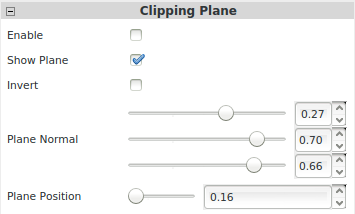
\includegraphics[scale=0.6,keepaspectratio=true]{./images/clipplane_properties.png}
 % clipplane_properties.png: 355x214 pixel, 72dpi, 12.52x7.55 cm, bb=0 0 355 214
 \caption{The property group of a clipping plane. Click on the `Enable'-checkbox to activate the clipping.}
 \label{fig:clipplane_properties}
\end{figure}

The `\verb|Enable|'-checkbox can be used to enable or disable the clipping. By using the `\verb|Invert|'-checkbox, the normal vector
of the clipping plane is inverted, simply inverting the clipping direction. The `\verb|Plane Normal|' and `\verb|Plane Position|' settings
allow direct manipulation of the settings of the plane. This is, however, not a very intuitive way to control the orientation and position
of a plane in three-dimensional space. Instead, the user can activate a plane widget in the three-dimensional view by using the 
`\verb|Show Plane|'-checkbox. The plane manipulation widget includes a handle for direct interaction with the clipping plane 
by using the mouse in the three-dimensional view of the quad view. This does also work while the three-dimensional view
is enlarged. An example is depicted in figure \ref{fig:planemanipulation}.

\begin{figure}[htb]
 \centering
 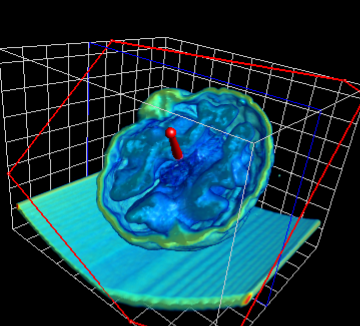
\includegraphics[scale=0.4,keepaspectratio=true]{./images/clipplane_handle.png}
 % clipplane_handle.png: 360x326 pixel, 72dpi, 12.70x11.50 cm, bb=0 0 360 326
 \caption{The clipping plane handle}
 \label{fig:planemanipulation}
\end{figure}

The clipping plane handle can be manipulated in various ways by the user. First, clicking and holding the left mouse button on the
shaft of the handle allows to move the clipping plane along the plane normal. By clicking and holding the left mouse button on the 
sphere at the end of the handle, the plane can be rotated around the center of the handle. Clicking and holding the right mouse 
button anywhere on the handle allows to move the handle on the clipping plane itself, which can be useful to get the right angle for a rotation.
While interacting with the clipping plane handle, the plane is rendered slightly transparent. 
This is depicted in figure \ref{fig:clipplane_manipulation}. While the `\verb|Show Plane|'-checkbox is 
activated, the position of the clipping plane is also indicated by several colored line segments which represent the intersection 
of the clipping plane with the bounding box of the data set, as can be seen in figure \ref{fig:planemanipulation}.

\begin{figure}[h]
 \centering
 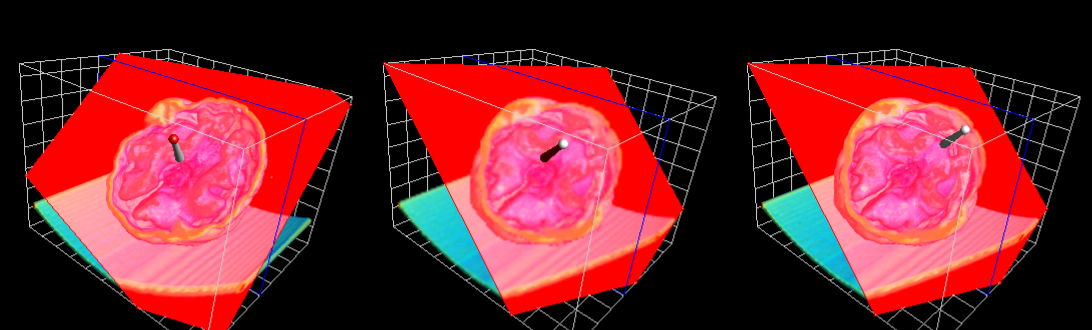
\includegraphics[scale=0.4,keepaspectratio=true]{./images/clipplane_manipulation.png}
 % clipplane_manipulation.png: 1092x330 pixel, 72dpi, 38.52x11.64 cm, bb=0 0 1092 330
 \caption{Clicking and holding the left mouse button on the shaft of the handle moves the plane (left image), clicking and holding the left mouse
 button on the sphere allows to rotate the plane (middle image), clicking and holding the right mouse button on the handle moves it along the plane 
 (right image).}
 \label{fig:clipplane_manipulation}
\end{figure}


\subsection{Animations}
\label{section:animation_editor}

It has already been mentioned in section \ref{section:interface} that the rightmost icon in the \Voreen tool bar opens and closes an animation editor.
Aside from the \Voreen startup workspace, which has a pre-defined example animation, the animation of a \workspace should be empty and the animation 
editor should look similar to figure \ref{fig:animation_window}.

\begin{figure}[htb]
 \centering
 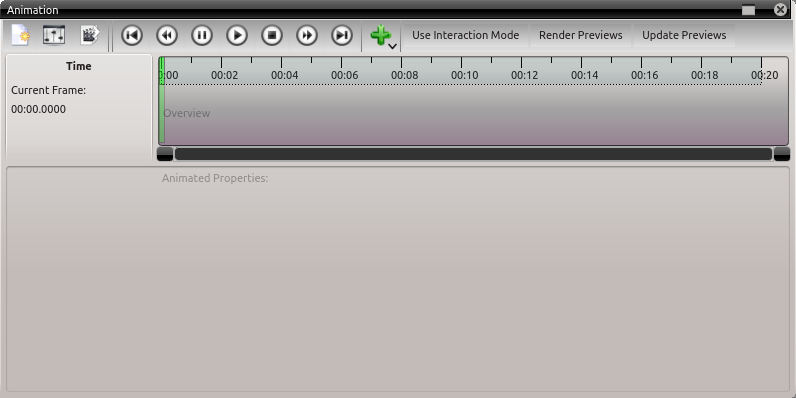
\includegraphics[scale=0.5,keepaspectratio=true]{./images/animation_window.png}
 % animation_window.png: 796x399 pixel, 90dpi, 22.47x11.26 cm, bb=0 0 637 319
 \caption{The animation window with an empty animation}
 \label{fig:animation_window}
\end{figure}

The animation editor consists of three basic parts. The first part is the animation tool bar, which is located at the top of the editor. Below the tool bar is the 
animation timeline, which provides an overview of the animation. The bottom part displays information and settings, depending on the current state of the animation
editor. 

\subsubsection{Creating a Basic Animation}
To animate a property, click on the `+'-button in the middle of the animation tool bar. It will open a menu where you can select one of the groups 
which are present in the property list window. Within the group, you can select one of the properties of that group. Clicking on the property will add 
it to the list of animated properties. If no animated property has been present in the animation before, the editor will also add a \emph{keyframe} to the
timeline. Basically every property which is present in the current workspace can be added to the animation and be animated by setting a state for the property
in each of the animation keyframes. When playing back the animation, the current value for each frame is generated by interpolating between adjacent keyframes and 
setting it to the actual properties of the workspace, so that the result can directly be seen in the quad view rendering.

After adding the first property to the animation, the animation window should look similar to the one depicted in figure \ref{fig:animation_keyframe}.

\begin{figure}[!htb]
 \centering
 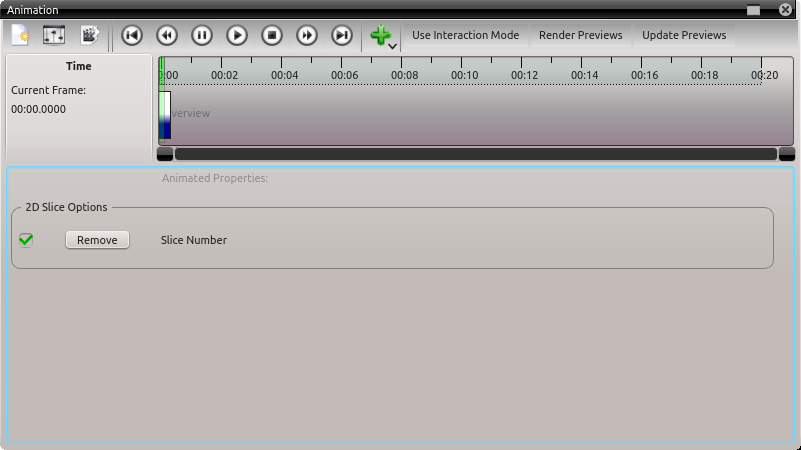
\includegraphics[scale=0.5,keepaspectratio=true]{./images/animation_keyframe.png}
 % animation_keyframe.png: 801x450 pixel, 90dpi, 22.61x12.70 cm, bb=0 0 641 360
 \caption{The animation window after a property has been added}
 \label{fig:animation_keyframe}
\end{figure}

The area at the bottom of the animation window now displays a list of all of the animated properties for each group. The property can be removed from the animation by using the 
`\verb|Remove|'-button. However, this will erase all of its animation state from the animation. By clicking the checkbox to the left of the button, animating the property
can be deactivated while still keeping the values set to the animation keyframes. Clicking on the checkbox of a deactivated property will activate its animation again.

By clicking on the keyframe in the timeline, it can be selected. This will change the layout of the bottom section of the animation window so that the value of each  
animated property can be edited for this keyframe. An example of this with two animated properties is depicted in figure \ref{fig:animation_keyframe_editing}.

\begin{figure}[htb]
 \centering
 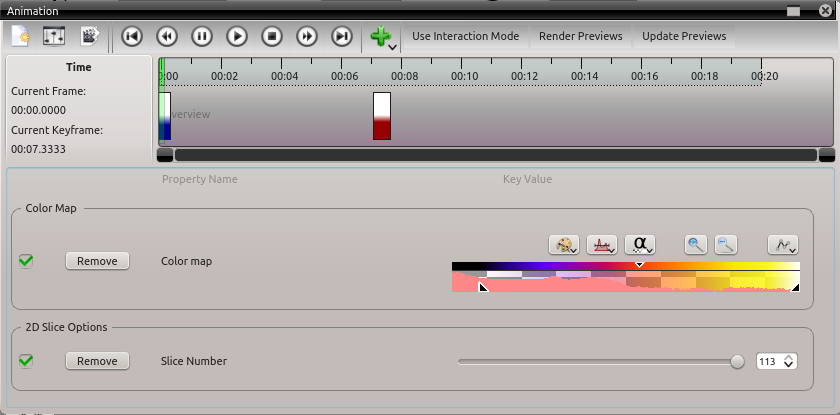
\includegraphics[scale=0.5,keepaspectratio=true]{./images/animation_keyframe_editing.png}
 % animation_keyframe_editing.png: 840x415 pixel, 90dpi, 23.71x11.71 cm, bb=0 0 672 332
 \caption{Editing the property values of a keyframe}
 \label{fig:animation_keyframe_editing}
\end{figure}

To add another keyframe to the animation, right-click on the lower part of the animation timeline (i.e. the part where the keyframes are located) and select either
`\verb|Add Keyframe|' or `\verb|Take Snapshot|'. The first option will create a keyframe, where the values for all of its animated properties are computed by interpolating 
between the keyframes already present (or using the value of the first or last keyframe, if the new keyframe is inserted as the first or last in the timeline). The 
second option will use the values currently set in the \Voreen application and record those to a keyframe. This is especially useful for three-dimensional camera settings,
as you can position the camera and then record the state to the animation.

By clicking on a keyframe and holding the left mouse button, the keyframe can be moved in the timeline. Right-clicking on a keyframe opens a menu where the keyframe 
can be removed from the animation or a snapshot of the current application settings can be recorded to the existing keyframe, overwriting its former values.

Clicking with the left mouse button in the space between two keyframes in the timeline allows to select the interval between those keyframes. 
An example of this is depicted in figure \ref{fig:animation_interval}.
\begin{figure}[!htb]
 \centering
 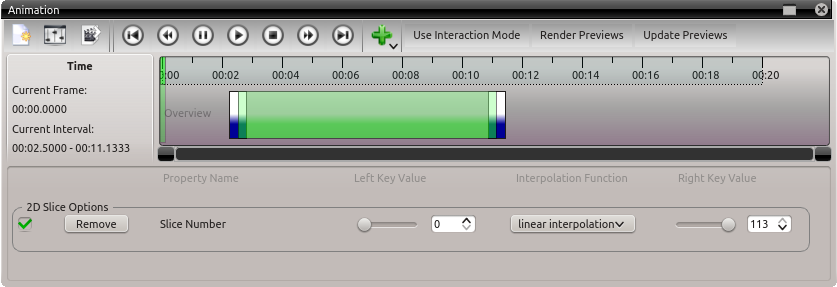
\includegraphics[scale=0.5,keepaspectratio=true]{./images/animation_interval.png}
 % animation_interval.png: 837x287 pixel, 90dpi, 23.62x8.10 cm, bb=0 0 670 230
 \caption{Selecting an interval between two keyframes of the animation}
 \label{fig:animation_interval}
\end{figure}
Selecting an interval, similar to selecting a single keyframe, allows to change the value of each of the animated properties for both the left and right keyframe.
Additionally, you can change the interpolation function that is used to interpolate between the keyframes within the interval. In most cases, the default linear 
interpolation will be sufficient. For camera animations, however, a \emph{spherical linear interpolation} should be selected.\footnote{The same
usually goes for the orientation of a clipping plane.}

The top part of the animation timeline allows to set the \emph{frame marker} to a specific time by clicking on it with the left mouse button. This will also set
the state of the animation at this time to the application, so that it allows to inspect the state of the animated properties at a specific time of the animation
directly using the quad view. Holding the left mouse button while moving in the top part of the animation timeline allows to scan through the animation, while
the state of the animated properties is directly set to the application properties. Figure \ref{fig:animation_marker} shows an example of this.

\begin{figure}[htb]
 \centering
 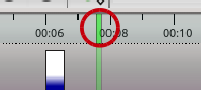
\includegraphics[scale=0.8,keepaspectratio=true]{./images/animation_marker1.png}
 % animation_marker1.png: 201x90 pixel, 96dpi, 5.32x2.38 cm, bb=0 0 151 67
 \caption{Clicking in the top part of the timeline (marked by the red circle) will set the current frame.}
 \label{fig:animation_marker}
\end{figure}

\subsubsection{The Animation Tool Bar}

The leftmost icon of the animation tool bar will create a new, empty animation. However, this will erase all of the animation settings currently 
present. Animations are part of the workspace setting. It is therefore necessary to save the workspace if you want to save the animation. Animations
cannot be saved independently, as they operate on the workspace-specific properties and settings.

\begin{figure}[!htb]
 \centering
 
\includegraphics[scale=0.7,keepaspectratio=true]{./images/animation_toolbar.png}
 % animation_toolbar.png: 735x32 pixel, 90dpi, 20.75x0.90 cm, bb=0 0 588 26
 \caption{The animation tool bar}
 \label{fig:animation_toolbar}
\end{figure}

The second tool bar icon opens an animation settings dialog, which is depicted in figure \ref{fig:animation_settings}. In this dialog, you can set the duration
of the animation, i.e. the length of the animation timeline where keyframes can be placed. By selecting the `\verb|Apply Time Stretch|'-checkbox, the current
animation is scaled to fit the new duration. This can be useful to speed up or slow down an already existing animation.

\begin{figure}[htb]
 \centering
 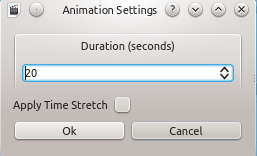
\includegraphics[scale=0.7,keepaspectratio=true]{./images/animation_settings.png}
 % animation_settings.png: 257x156 pixel, 90dpi, 7.25x4.40 cm, bb=0 0 206 125
 \caption{The animation settings dialog window}
 \label{fig:animation_settings}
\end{figure}

Next to the animation settings icon is the export icon, which opens the export dialog window depicted in figure \ref{fig:animation_export}. 
It allows to export the animation as a frame sequence, i.e. a sequence of `\verb|*.png|'-image files, or as a video file, and offers several configuration
options for the export format, quality and compression.

\begin{figure}[!htb]
 \centering
 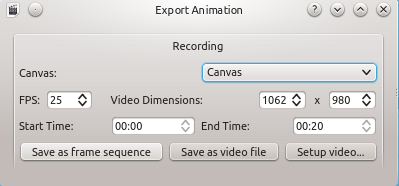
\includegraphics[scale=0.7,keepaspectratio=true]{./images/animation_export.png}
 % animation_export.png: 399x186 pixel, 90dpi, 11.26x5.25 cm, bb=0 0 319 149
 \caption{The animation export window}
 \label{fig:animation_export}
\end{figure}

Next to the export icon on the animation tool bar are the animation playback control icons, which offer the functionality to play, pause, and stop the animation playback, etc.

Activating the `\verb|Use Interaction Mode|'-button will use an interaction mode with reduced rendering quality during playback to improve the rendering speed 
of the animation. The `\verb|Use Interaction Mode|'-button activates the display of a series of small images on the timeline which visualize the animation state.
The preview images are not updated automatically if the animation changes after the previews have been created. 
The user therefore has to click on the `\verb|Update Previews|'-button to update
the preview images according to the current animation state.


\newpage 


